
\documentclass[11pt,a4paper]{article}

\usepackage[utf8]{inputenc}
\usepackage[T1]{fontenc}
\usepackage[spanish]{babel}

\usepackage{tgpagella}
\usepackage{geometry}
\usepackage{graphicx}
\usepackage{xcolor}
\usepackage{titlesec}
\usepackage{fancyhdr}
\usepackage[parfill]{parskip}
\usepackage[expansion=false]{microtype}
\usepackage{hyperref}
\usepackage{setspace}
\usepackage{needspace}

\geometry{top=3.0cm,bottom=3.0cm,left=3.5cm,right=3.5cm}

\setlength{\parskip}{0.65em}
\setlength{\parindent}{0em}

\definecolor{azulai}{RGB}{30,80,140}
\definecolor{doradoai}{RGB}{140,90,0}
\definecolor{grisai}{RGB}{70,70,70}

\titleformat{\section}
{\Large\bfseries\color{azulai}}
{}{0em}{}
[{\color{azulai}\titlerule[0.5pt]}]

\titlespacing*{\section}{0pt}{1.8em}{0.8em}

\titleformat{\subsection}
{\large\bfseries\color{doradoai}}
{}{0em}{}

\titlespacing*{\subsection}{0pt}{1.2em}{0.4em}

\pagestyle{fancy}
\fancyhf{}

\rhead{\textcolor{grisai}{\small Prueba — Arquitectura Interna}}
\lhead{\textcolor{grisai}{\small Carta Natal Base}}

\cfoot{\textcolor{grisai}{\small\thepage}}

\renewcommand{\headrulewidth}{0.3pt}

\hypersetup{
colorlinks=true,
linkcolor=azulai,
urlcolor=azulai
}

\setstretch{1.4}

\begin{document}

% ── PORTADA ──────────────────────────────────────────────────────────────

\begin{titlepage}

\centering

\vspace*{1.5cm}

{\Huge\bfseries\color{azulai} Carta Natal Base}\\[0.5cm]

{\large\color{grisai} Arquitectura Interna}\\[0.4cm]

{\small\itshape\color{grisai}
Un método para sostener cuerpo, energía y vida con coherencia
}\\[2cm]

{\huge\color{doradoai} Prueba}\\[1.5cm]

{\Large 16/04/2026 \quad 00:35}\\[0.3cm]

{\Large Gernika-Lumo, España}\\[0.3cm]

{\normalsize
Lat: 43.3144° \quad
Lon: -2.6779° \quad
UTC+02:00
}\\[0.5cm]

{\normalsize
Ascendente: Sagitario 9°35'
}\\[2.5cm]

\vfill

{\small Generado el 21/05/2026}

\end{titlepage}


% ── INTRODUCCIÓN ─────────────────────────────────────────────────────────────

\section*{Introducción}

Esta carta natal base no busca definir quién eres.

La astrología se utiliza aquí como lenguaje de observación:
una forma de mirar cómo se organiza tu energía,
qué registros aparecen con más facilidad
y qué dinámicas pueden influir en tu manera de vivir, sostenerte y relacionarte con el entorno.

No se trata de una lectura predictiva ni de una identidad fija.
Es un mapa inicial de orientación.

Las siguientes páginas muestran únicamente las capas principales de la carta:
los ejes más visibles,
la distribución general de la energía
y algunos patrones básicos desde los que sueles moverte.

\vspace{0.4cm}

\newpage


% ── RUEDA ────────────────────────────────────────────────────────────────

\section{Carta Natal}

\begin{center}
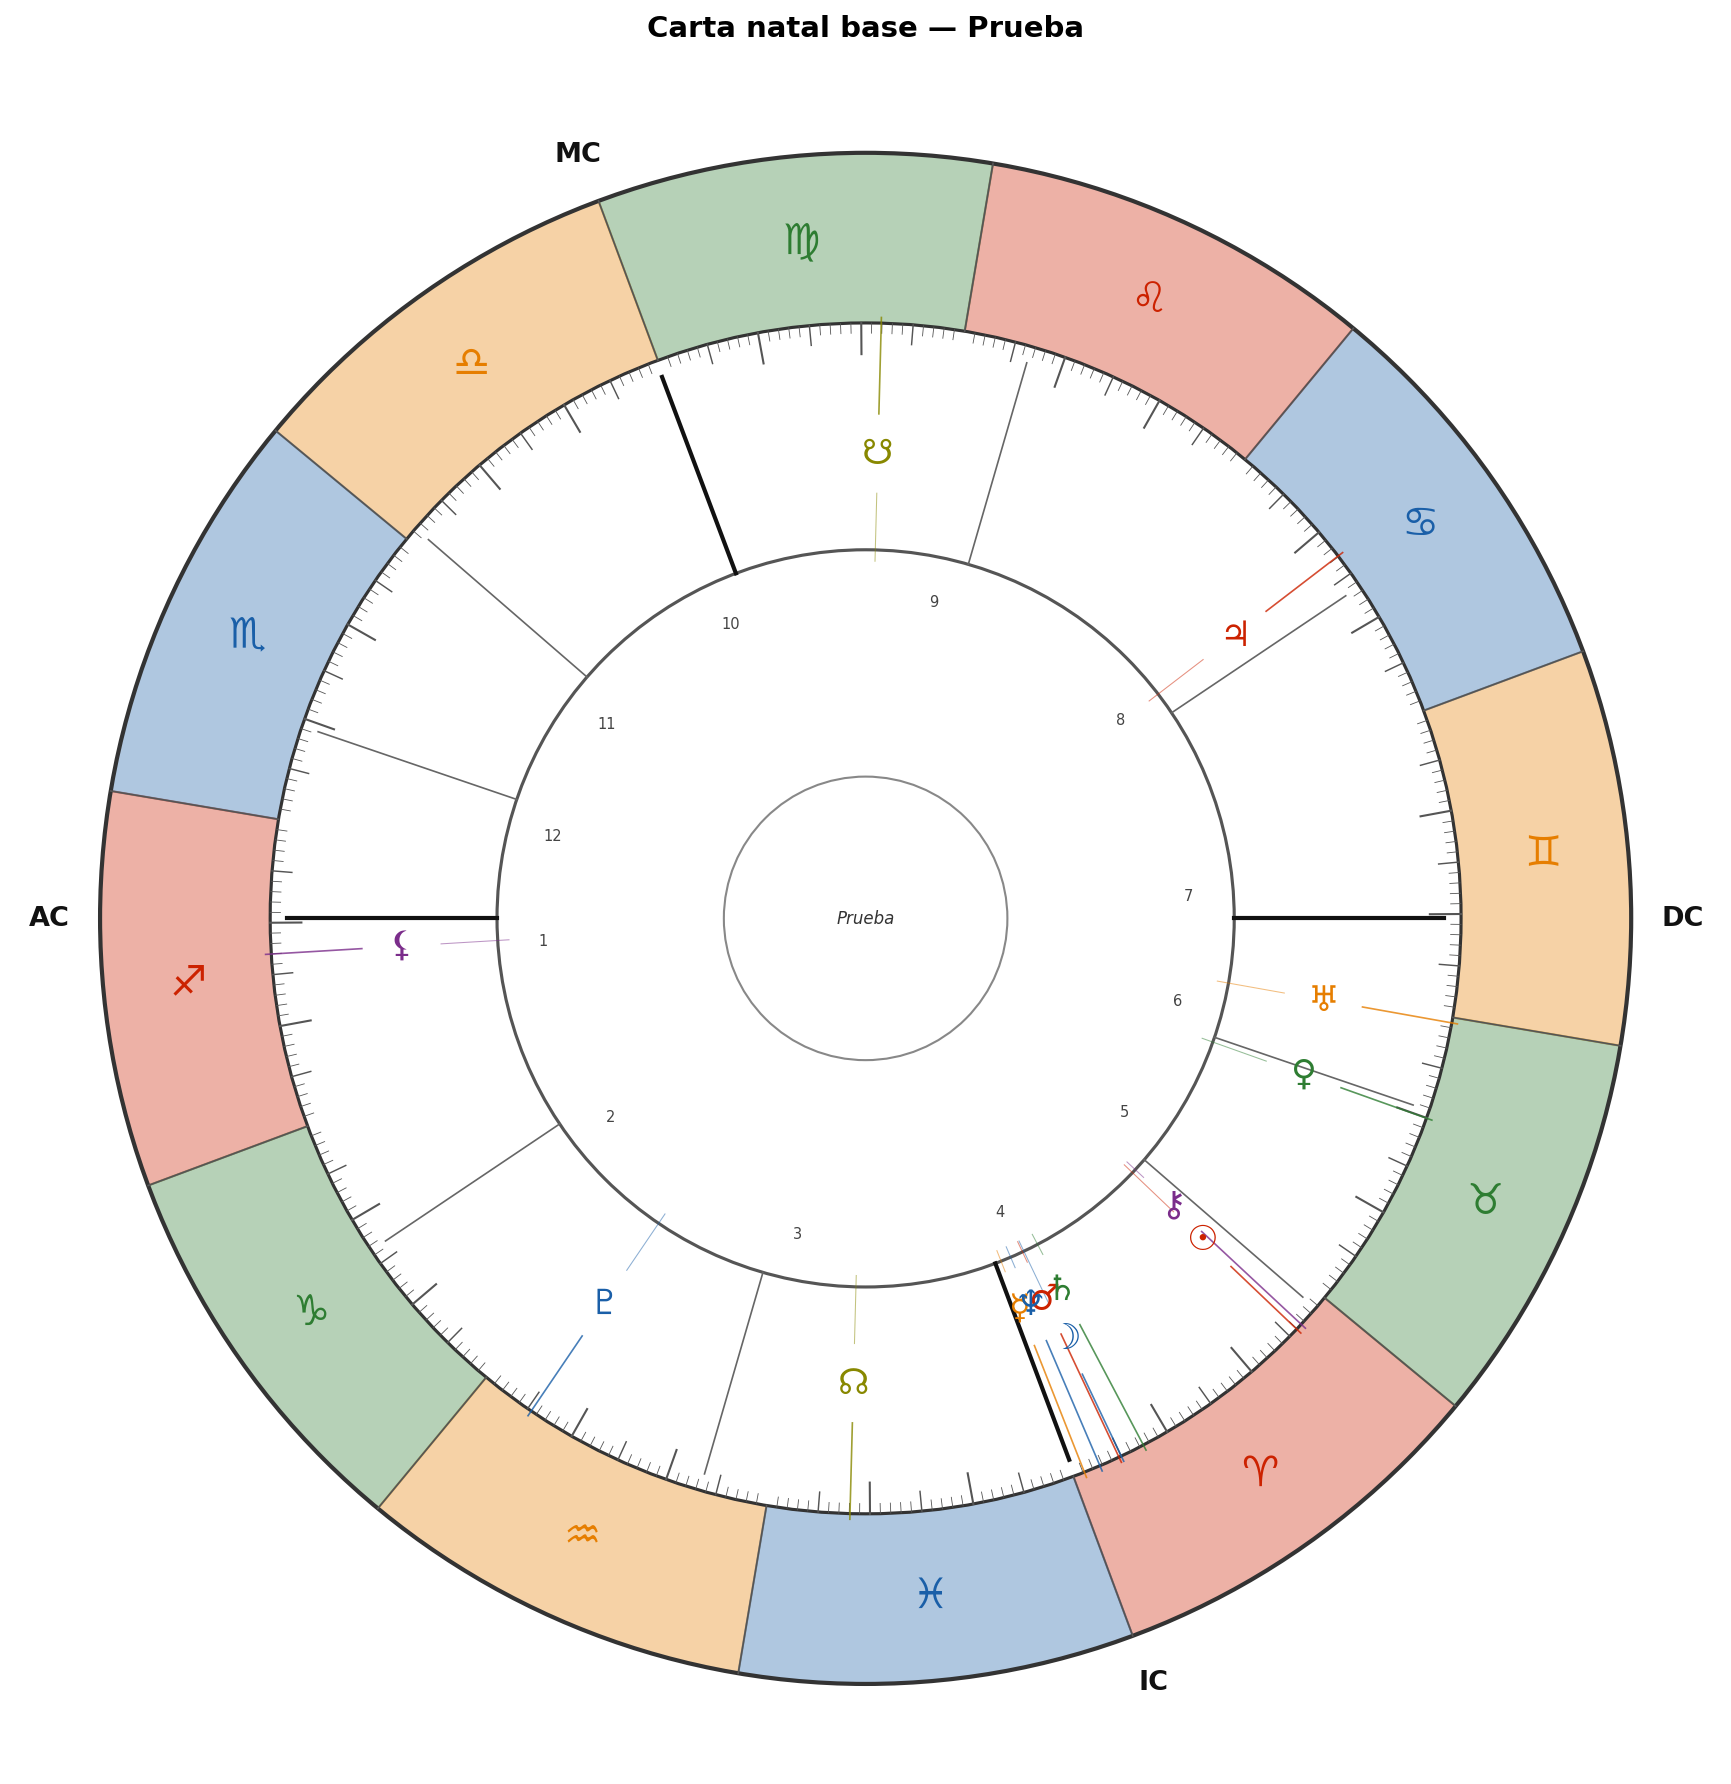
\includegraphics[width=0.8\textwidth]{Prueba_carta_base_rueda.png}
\end{center}

\vspace{0.8cm}

% ── POSICIONES PRINCIPALES ───────────────────────────────────────────────

\section{Posiciones principales}

\begin{center}

Sol en Aries — Casa 4\\
Luna en Aries — Casa 4\\
Ascendente Sagitario\\
Medio Cielo en Libra

\end{center}

\vspace{0.5cm}

{\small\itshape
La lectura ampliada desarrolla el mapa completo de posiciones,
aspectos y configuraciones de la carta.
}

\vspace{0.8cm}
\Needspace{5\baselineskip}

% ── VISIÓN GENERAL ───────────────────────────────────────────────────────

\section{Visión general}

Tu carta muestra esta distribución de elementos: Fuego 11, Tierra 2.5, Aire 1, Agua 2. El elemento más presente es Fuego (iniciativa, impulso y necesidad de movimiento). Esto señala un registro que suele aparecer con facilidad en tu forma de funcionar. El elemento menos presente es Agua (sensibilidad, percepción emocional y conexión con el entorno) y Aire (pensamiento, comunicación y necesidad de perspectiva). No significa ausencia, sino una cualidad que puede necesitar más atención consciente. Predomina la modalidad cardinal, asociada a la iniciativa, el comienzo y la capacidad de activar procesos. Tu Medio Cielo en Libra orienta tu presencia pública hacia la equilibrio, mediación y capacidad de relación.

\vspace{0.8cm}
\Needspace{5\baselineskip}


% ── LECTURA DE LOS ELEMENTOS ────────────────────────────────────────────

\section{Lectura de los elementos}

\subsection{Aire bajo}

No pasas tanto por la cabeza. Tiendes a ir directa a lo que haces o sientes sin pensarlo mucho. Puede costar ordenar ideas o explicar lo que te pasa.

\textbf{Observa:}
\begin{itemize}
\item si te cuesta explicar lo que sientes o piensas
\item si necesitas más tiempo para entender lo que te ocurre
\item en qué momentos te vendría bien parar y pensar un poco
\end{itemize}

\vspace{0.4cm}
\Needspace{5\baselineskip}

\subsection{Tierra equilibrado}

Puedes organizarte y también adaptarte. Sabes cuándo mantener algo y cuándo cambiarlo.

\textbf{Observa:}
\begin{itemize}
\item cómo te organizas en tu día a día
\item cuándo mantienes algo aunque ya no sirve
\item cuándo cambias sin problema
\end{itemize}

\vspace{0.4cm}
\Needspace{5\baselineskip}

\subsection{Agua bajo}

No siempre conectas fácilmente con lo que sientes. Puede costar identificar o expresar emociones.

\textbf{Observa:}
\begin{itemize}
\item si te cuesta saber qué estás sintiendo
\item si evitas lo emocional
\item en qué momentos conectas más con ello
\end{itemize}

\vspace{0.4cm}
\Needspace{5\baselineskip}

\subsection{Fuego alto}

Tienes mucha energía para actuar. Te mueves rápido y tomas iniciativa. Puedes ir demasiado deprisa o no sostener lo que empiezas.

\textbf{Observa:}
\begin{itemize}
\item si te lanzas sin pensar
\item si empiezas cosas y luego las dejas
\item cuándo necesitas bajar el ritmo
\end{itemize}

\vspace{0.4cm}
\Needspace{5\baselineskip}

\subsection{Integración}

Esto no define quién eres. Solo muestra cómo tiendes a funcionar.

No hay nada que cambiar. Se trata de verlo y aprender a manejarlo mejor.

\vspace{0.4cm}

\begin{center}
{\small\itshape
Ten en cuenta que tienes que hacer la amalgama de todos los elementos. Por ejemplo, si tienes Fuego muy alto pero también mucha Tierra, puede que no dejes proyectos a medias.
}
\end{center}


\vspace{0.8cm}
\Needspace{10\baselineskip}


% ── LOS TRES PILARES ────────────────────────────────────────────────────

\section{Los tres pilares}

\Needspace{14\baselineskip}
\subsection{Sol en Aries}

Con el Sol en Aries, necesitas movimiento, iniciativa y sensación de avance. Tu energía suele activarse rápidamente cuando algo te entusiasma o supone un reto. Muchas veces funcionas mejor actuando y corrigiendo sobre la marcha que esperando demasiado tiempo. Con el Sol en Casa 4, la intimidad, la sensación de hogar y la vida interior suelen tener mucho peso en tu desarrollo. Necesitas espacios donde puedas bajar la guardia y sentir cierta seguridad emocional. Muchas veces lo privado o lo emocional influye más en ti de lo que otras personas perciben desde fuera.

\vspace{0.8cm}
\Needspace{5\baselineskip}

\Needspace{10\baselineskip}
\subsection{Luna en Aries}

Con la Luna en Aries, las emociones suelen aparecer de forma rápida y directa. Necesitas sentir espacio, movimiento y capacidad de actuar cuando algo te afecta. Muchas veces te ayuda más hacer algo con lo que sientes que quedarte demasiado tiempo dándole vueltas. Con la Luna en Casa 4, la intimidad, el hogar y la sensación de protección emocional suelen ocupar un lugar muy importante en tu vida. El entorno cercano influye bastante en cómo te sientes y en tu capacidad de descansar realmente.

\vspace{0.8cm}
\Needspace{5\baselineskip}

\Needspace{10\baselineskip}
\subsection{Ascendente Sagitario}

Con Ascendente en Sagitario, normalmente te muestras de forma abierta, espontánea y bastante directa. Sueles entrar en los entornos con energía, entusiasmo o sensación de movimiento. Las demás personas suelen percibir facilidad para conectar y amplitud en tu forma de relacionarte.

\vspace{0.8cm}
\Needspace{5\baselineskip}

% ── CIERRE ───────────────────────────────────────────────────────────────

\section{Cierre}

Esta carta no busca definirte ni darte una identidad fija.

La astrología se utiliza aquí como lenguaje de observación:
una forma de mirar tendencias, ritmos y maneras de relacionarte con la vida.

La lectura ampliada desarrolla con más profundidad:
los vínculos,
la regulación emocional,
los patrones repetitivos,
la dirección de crecimiento,
las tensiones internas
y las configuraciones principales de la carta.

La lectura completa no busca darte más información.
Busca ayudarte a entender cómo sostener tu vida sin romperte por dentro.

\vspace{1cm}

\begin{center}

{\small\itshape\color{grisai}
Arquitectura Interna
}

\end{center}

\end{document}
